\documentclass{ctexart}
\usepackage{graphicx}
\usepackage{caption}
\usepackage{float}
\usepackage{amsmath}
\usepackage{fancyhdr}
\usepackage{xunicode-addon}
\usepackage{booktabs}
\usepackage{listings}
\usepackage{hyperref}
\usepackage[a4paper,hmargin=1.25in,vmargin=1in]{geometry}
% !TeX program = xelatex
\lstdefinestyle{mystyle}{
  basicstyle=\ttfamily\footnotesize,
  breakatwhitespace=false,         
  breaklines=true,                 
  captionpos=b,                    
  keepspaces=true,                 
  numbers=left,                    
  numbersep=5pt,                  
  showspaces=false,                
  showstringspaces=false,
  showtabs=false,                  
  tabsize=2
}

\lstset{style=mystyle}

\title{\begin{figure}[H]
	\centering 
	\includegraphics[height=7cm,width=14cm]{E:/Pictures/中科大.jpg}
	\end{figure}\Huge\textbf{数据结构实验报告2}\\\huge{栈与队列的应用}}
\date{}
\punctstyle{banjiao} 
\pagestyle{fancy}
	\fancyhead[C]{\LARGE\textbf{实验报告2}}
	\fancyhead[L]{}
	\fancyhead[R]{}
	\fancyfoot[C]{\thepage}
\begin{document}
	\maketitle
	\thispagestyle{empty}
	
	\[\makebox{\Large{姓名:\underline{\makebox[5cm]{高茂航}}}}\]
	
    \[\makebox{\Large{学号:\underline{\makebox[5cm]{PB22061161}}}}\]
	
	\[\makebox{\Large{日期:\underline{\makebox[5cm]{2023年10月30日}}}}\]
	
	\clearpage

	\pagenumbering{arabic}
\section{括号匹配检验}
	\subsection{问题描述}
	假设一个表达式有英文字母(大、小写)、数字、四则运算符(+,-,*,/)和左右小括号、中括号、大括号构成,以“@”作为表达式的结束符。
	请编写一个程序检查表达式中的左右大中小括号是否匹配,若匹配,则返回“Yes”;否则返回“No”。
	
	\subsection{算法描述}
	\subsubsection{数据结构}
	用链栈来储存尚未完成匹配的括号。
	\begin{lstlisting}[language=C++, caption=链栈相关操作]
	typedef struct StackList{
		char ope; //储存括号的链栈节点
		struct StackList* next;
	}Stack;
	Stack* PushStack(Stack** S,char c){//将括号进栈
		Stack *p=(Stack*)malloc(sizeof(Stack));
		p->ope=c;
		if(!*S){
			*S=p;
			(*S)->next=NULL;
		}
		else{
			p->next=*S;
			*S=p;
		}
		return *S;
	}
	char PopStack(Stack** S){//将栈顶括号出栈
		char c;
		Stack *p=*S;
		c=p->ope;
		(*S)=(*S)->next;
		free(p);
		return c;
	}
	char GetStackTop(Stack* S){//取栈顶括号
    if(!S)
        return 0;
    return S->ope;
}
	\end{lstlisting}
	\subsubsection{括号匹配检验算法}
	每次读到左括号就进栈,读到右括号就出栈,
	如果出栈的括号与读到的右括号不匹配,则返回“No”,如果最后栈为空,则返回“Yes”。
	\begin{lstlisting}[language=C++, caption=括号匹配检验算法]
		int BracketTest(char* a){//检验括号是否匹配
		int i=0;
		Stack* S=NULL;
		char x;
		while(a[i]&&a[i]!='@'){
			switch (a[i]) {
				case '(':
				case '[':
				case '{':
					PushStack(&S,a[i]);
					i++;			
					break;
				case ')':{
					if(!S)
						return 0;
					char c1=PopStack(&S);
					if(c1=='['||c1=='{')
						return 0;
					i++;	
					break;
				}
				case ']':{
					if(!S)
						return 0;
					char c2=PopStack(&S);
					if(c2=='{'||c2=='('||(GetStackTop(S)&&GetStackTop(S)=='('))//判断优先级
						return 0;
					i++;			
					break;
				}
				case '}':{
					if(!S)
						return 0;
					char c3=PopStack(&S);
					if(c3=='('||c3=='['||(GetStackTop(S)&&(GetStackTop(S)=='('||GetStackTop(S)=='[')))
						return 0;
					i++;			
					break;
				}
				default:{
					i++;
					break;
				}
			}
		}
		if(S)
			return 0;//最后栈不为空,说明有左括号没有匹配到右括号
		return 1;	
	}
	\end{lstlisting}
	\subsubsection{主函数(包括读取文件操作)}
	2.txt文件内容为:
	\begin{lstlisting}[language=C++, caption=2.txt]
	6
	3*(4+5)-{6/[7*(8-9)]}@
	{[1+2*(3-4)]/5}+6-7@
	1+[2*(3-4]}/5@
	6*{7+[8-(9*10]}@
	8/{9+(10-[11*12])}@
	{[(2+3*4]/(5-6)+7}@
	\end{lstlisting}
	\begin{lstlisting}[language=C++, caption=主函数]
	int main(){
		int n,i;
		FILE *fp=fopen("2.txt","r");
		if (!fp) {
			fprintf(stderr, "无法打开文件\n");
			return 0;
		}
		fscanf(fp, "%d", &n);
		fgetc(fp);//读掉换行符
		char st[10][50];
		for(i=0;i<n;i++)
			fgets(st[i],sizeof(st[i]),fp);//st[i]是第i个字符串
		for(i=0;i<n;i++){
			if(BracketTest(st[i]))
				cout<<"Yes"<<endl;
			else
				cout<<"No"<<endl;	
		}
		fclose(fp);
	}
	\end{lstlisting}
	\subsection{调试分析}
	1.进栈出栈函数形参没有设置为指向指针的指针以达到修改指针指向的目的;

	2.忽略了完成匹配后栈不为空的情况。
	\subsection{算法时空分析}
	由于采用栈的链式存储,所以空间复杂度和时间复杂度都为$O(n)$。
	\subsection{测试结果}
	\begin{figure}[H]
		\centering 
		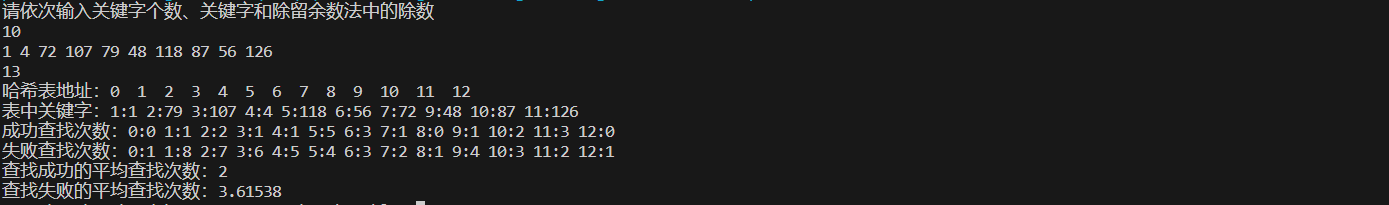
\includegraphics[height=4cm,width=6cm]{1.png}
		\end{figure}

\section{银行业务模拟}
	\subsection{问题描述}
	银行客户业务分为两种:第一种是申请从银行得到一笔资金,即取款或借款;第二种是向银行投入一笔资金,即存款或还款。

	银行有两个服务窗口,相应地有两个队列。客户到达银行后先排第一个队,处理每个客户业务时,如果属于第一种,且申请额超出银行现存资金总额而得不到满足,则立刻排入第二个队等候直至满足时才离开银行;否则业务处理完后立刻离开银行,每接待完一个第二种业务的客户,则顺序检查和处理(如果可能)第二个队列中的客户,对能满足的申请者予以满足,不能满足者重新排到第二个队列的队尾。注意,在此检查过程中,一旦银行资金总额少于或等于刚才第一个队列中最后一个客户(第二种业务)被接待之前的数额,或者本次已将第二个队列 检查或处理了一遍,就停止检查(因为此时已不可能还有能满足者),转而继续接待第一个队列的客户。任何时刻都只开一个窗口。假设检查不需要时间,营业时间结束时所有客户立即离开银行。
	写一个上述银行业务的事件驱动模拟系统,通过模拟方法求出客户在银行内逗留的平均时间。
	\subsection{算法描述}
	\subsubsection{数据结构}
	\begin{lstlisting}[language=C++, caption=链队列基本操作]
	typedef struct QueueList{
		int num; //顾客序号
		struct QueueList* next;
	}Queue;
	Queue* EnQueue(Queue** Q,int n){//将顾客进队
		Queue *p=(Queue*)malloc(sizeof(Queue));
		p->num=n;
		if(!*Q){
			*Q=p;
			(*Q)->next=NULL;
		}
		else{
			Queue* q=*Q;
			while(q->next)
				q=q->next;
			q->next=p;
			p->next=NULL;
		}
		return *Q;
	}
	int DeQueue(Queue** Q){//将队首顾客出队
		if(!*Q)
			return -1;
		int i;
		Queue *p=*Q;
		i=p->num;
		*Q=(*Q)->next;
		free(p);
		return i;
	}
	\end{lstlisting}
	\subsubsection{模拟过程}
	\begin{lstlisting}[language=C++, caption=模拟过程]
	int main(){
		int n,i,arrive[50]={0},status[50],Time=0,wait[50]={0},waittotal=0,waitaverage=0,closetime=0,avetime=0,Money=0,money[50]={0},moneytemp=0;
		//n为顾客人数,arrive数组记录每个顾客来到银行的时间,status数组记录每个顾客的状态,-1为没来银行,0为正在等待,1为已离开
		//Time表示当前时间,wait数组记录每个顾客等待的时间,waittotal是所有顾客等待的总时间,waitaverage是顾客等待的平均时间,closetime是银行关门时间,avetime是每笔交易的平均时间
		//Money为银行一开始的款额,money数组记录每个顾客的交易金额,正数为存钱,负数为取钱,moneytemp用来记录第一个队列最后一个客户(第二种业务)接待前银行的剩余款额
		cin>>n>>Money>>closetime>>avetime;
		Queue* Q=NULL;
		for(i=0;i<n;i++){
			cin>>money[i]>>arrive[i];
			status[i]=-1;
		}
		for(i=0;i<n;i++){
			if (arrive[i]>=closetime-avetime) {//在关门前完成不了交易相当于一直等到关门
				status[i]=0;
				break;
			}
			else {
				if(Time<arrive[i])
					Time=arrive[i];//重置当前时间
				if(money[i]<0){//第一种业务:取钱
					if(-money[i]<=Money){//银行有足够余额
						Money+=money[i];
						wait[i]=Time-arrive[i];
						status[i]=1;
						Time+=avetime;//重置当前时间
						moneytemp=Money;
						if(Time>=closetime)
							loop:break;
					}
					else{//银行没有足够余额,进入第二条队等待
						status[i]=0;
						EnQueue(&Q,i);
					}
				}
				else{//第二种业务
					Money+=money[i];
					wait[i]=Time-arrive[i];
					status[i]=1;
					Time+=avetime;//重置当前时间
					int status2[50]={0};//用来标记第二条队的顾客是否被检查到,没检查是0,检查到是1
					while (Money>moneytemp){
						int k=DeQueue(&Q);
                	if(k==-1) break;
                	else if(!status2[k]){
						if(-money[k]<=Money){
							Money+=money[k];
							wait[k]=Time-arrive[k];
							status[k]=1;
							Time+=avetime;//重置当前时间
							moneytemp=Money;
							if(Time>=closetime)
								goto loop;//跳出while循环和for循环
						}
						else{
							status2[i]=1;
							EnQueue(&Q,i);//不满足就重新入队
						}
					}
				}
			}
		}
	}
		for ( i = 0; i < n; i++){
			if(!status[i])
				wait[i]=closetime-arrive[i];
			cout<<"第"<<i+1<<"个顾客的等待时间为"<<wait[i]<<endl;
		}
		for ( i = 0; i < n; i++)
			waittotal+=wait[i];
		waitaverage=waittotal/n;
		cout<<n<<"个顾客的平均等待时间为"<<waitaverage<<endl;
	}
	\end{lstlisting}
	
	\subsection{调试分析}
出现问题不多,关键在于理清事件发生的逻辑,并注意时间的标记。
	\subsection{算法时空分析}
由于采用队列的链式存储,所以空间复杂度和时间复杂度都为$O(n)$。
	\subsection{测试结果分析}
	\begin{figure}[H]
		\centering 
		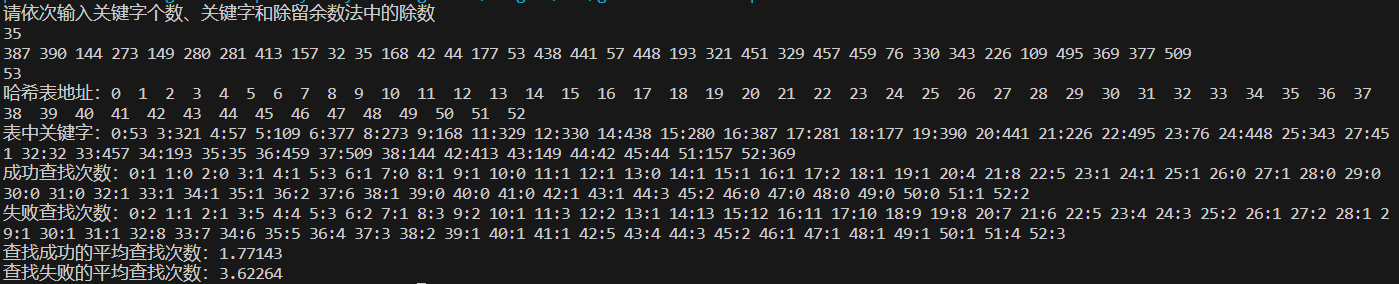
\includegraphics[height=6cm,width=14cm]{2.png}
		\end{figure}
		~1~号顾客~0~时刻到达银行,于~10~时办理完手续离开,此时银行有款额~8000~元;
		~2~号顾客~10~时刻到达银行,此时银行内存款不足,进入队列~2~;
		~3~号顾客~30~时刻到达银行,此时银行内存款不足,进入队列~2~;
		~4~号顾客~50~时刻到达银行,于~60~时办理完手续离开,此时银行有款额~10000~元。
		这时扫描队列~2~,队列~2~中第一个顾客~2~号顾客的要求仍然不满足,~2~号顾客出队再入队;
		此时队列~2~中第一个顾客~3~号客户满足要求,因此~3~号顾客于~60~时刻开始办理手续,于~70~时刻办理完毕离开银行,等待时间为$60-30=30$,此时银行有余款~0~元。
		然后直到银行关门时间~600~时刻~2~号客户都没有离开银行,等待时间为$600-10=590$。
	\section{实验体会收获}
加深了对栈和队列结构的理解,也对栈和队列的相关操作更加熟悉,并对栈和队列的应用有了更深的认识,此外也复习了读取文件的基本操作。
\end{document}